\documentclass[a4paper, 11pt]{article}
\usepackage[utf8]{inputenc}
\usepackage[margin=2.5cm]{geometry}
\usepackage{graphicx}
\usepackage{hyperref}
\usepackage{xcolor}
\usepackage{amsmath}
\usepackage{indentfirst}

\fboxsep=2pt
\fboxrule=0.8pt

\renewcommand*\contentsname{Table des matières}
\renewcommand{\familydefault}{\sfdefault}

\title{
	\hrulefill 
	\\
	Manuel d'utilisation 
	\\
	\textbf{Guardians Studio}
	
	\hrulefill
}

\date{EPITA Lyon $|$ Promo 2026}
\author{Alexandre Privat - Erwann Lesech - Guillaume Jolivalt - Raphaël Heng}

\begin{document}
	\maketitle
	
	\begin{figure}[ht]
		\centering
		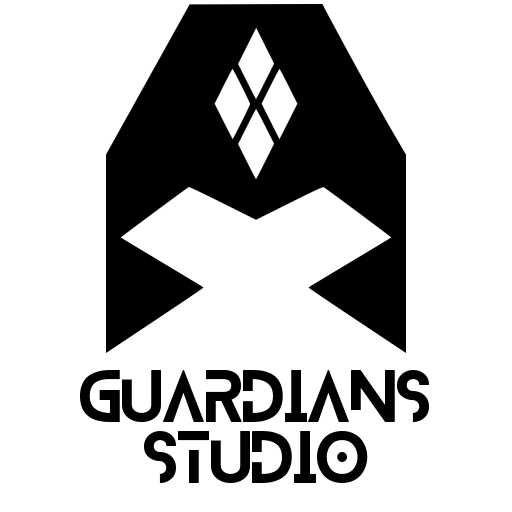
\includegraphics[width=10cm, height=10cm]{images/logo.png}
	\end{figure}
	
	\clearpage
	\tableofcontents
	\clearpage
	
	\section{Menus et interface du jeu}
	\subsection{Menu Principal}
	
	\begin{figure}[!ht]
		\centering
		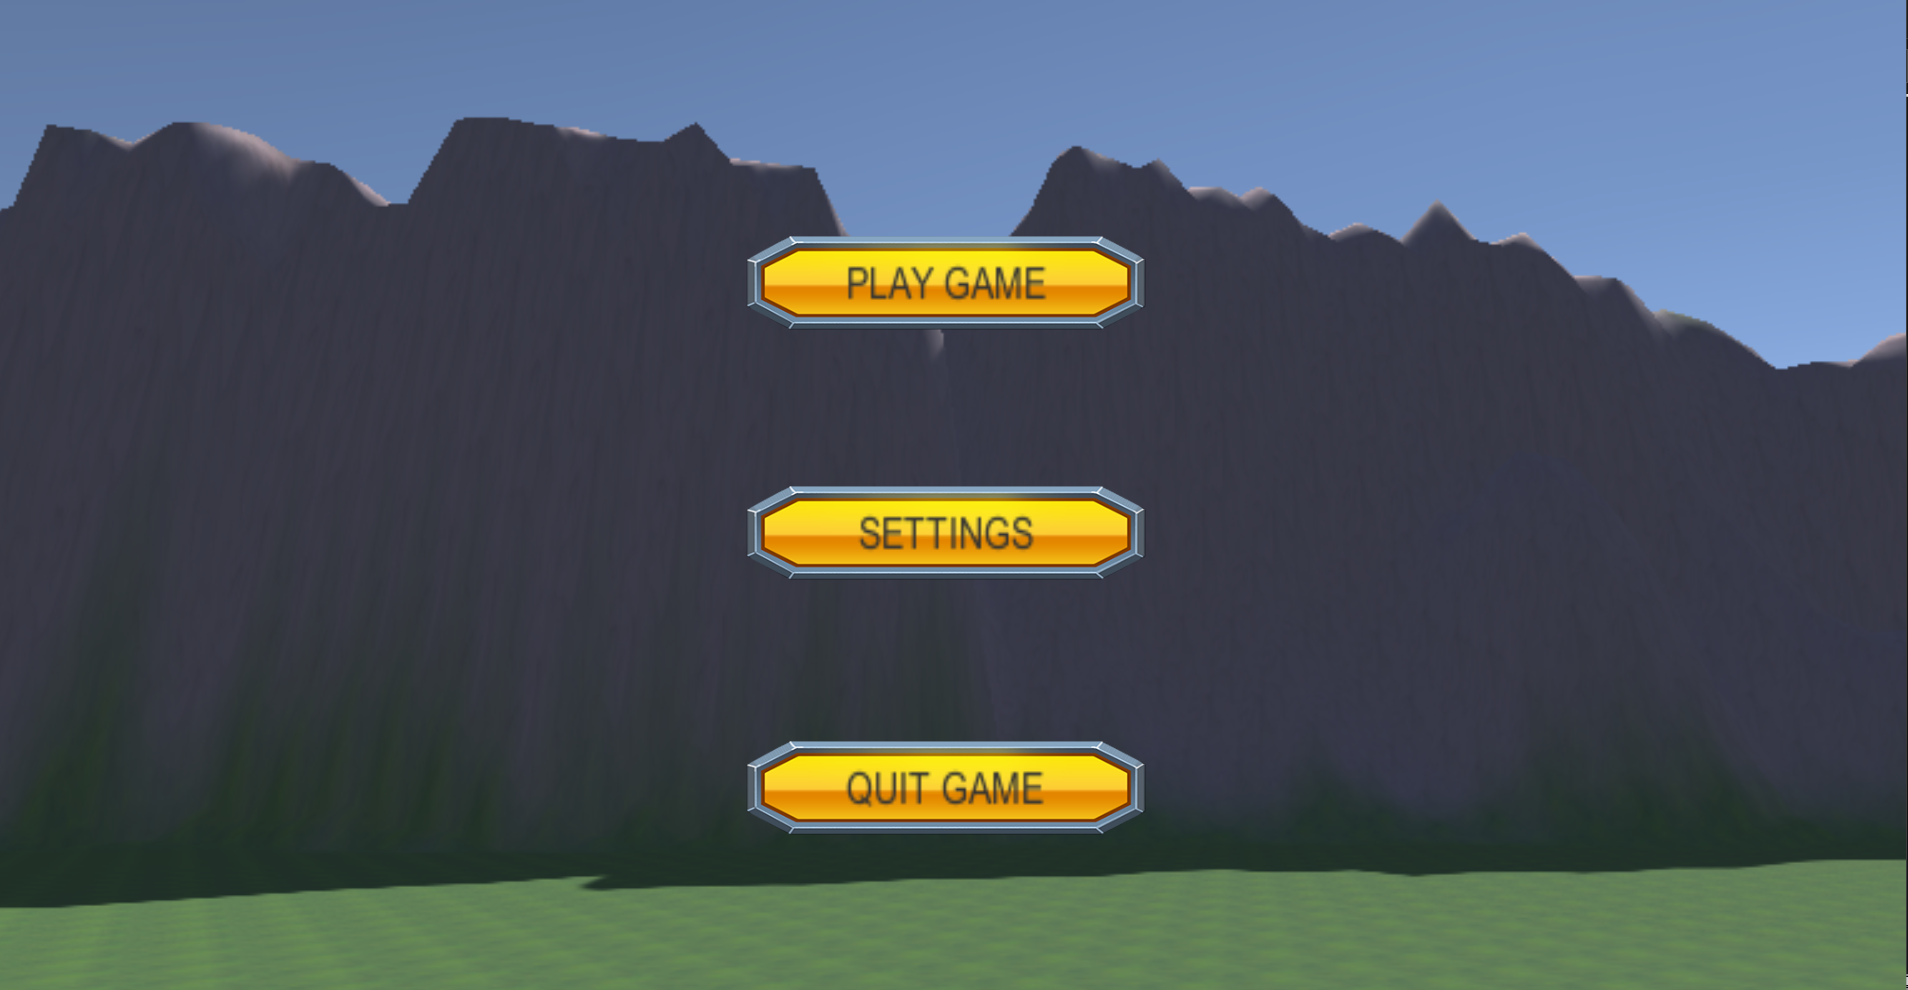
\includegraphics[scale=0.3]{images/menu_principal.png}
		\caption{Menu Principal}
	\end{figure}
	
	\noindent Dans ce menu, vous avez 3 options :
	\begin{itemize}
		\item Play Game : Lancer une partie en multijoueur ou en solo
		\item Settings : Aller dans les paramètres
		\item Quit Game : Quitter le jeu
	\end{itemize}
	
	\subsection{Menu Paramètres}
	\begin{figure}[!ht]
		\centering
		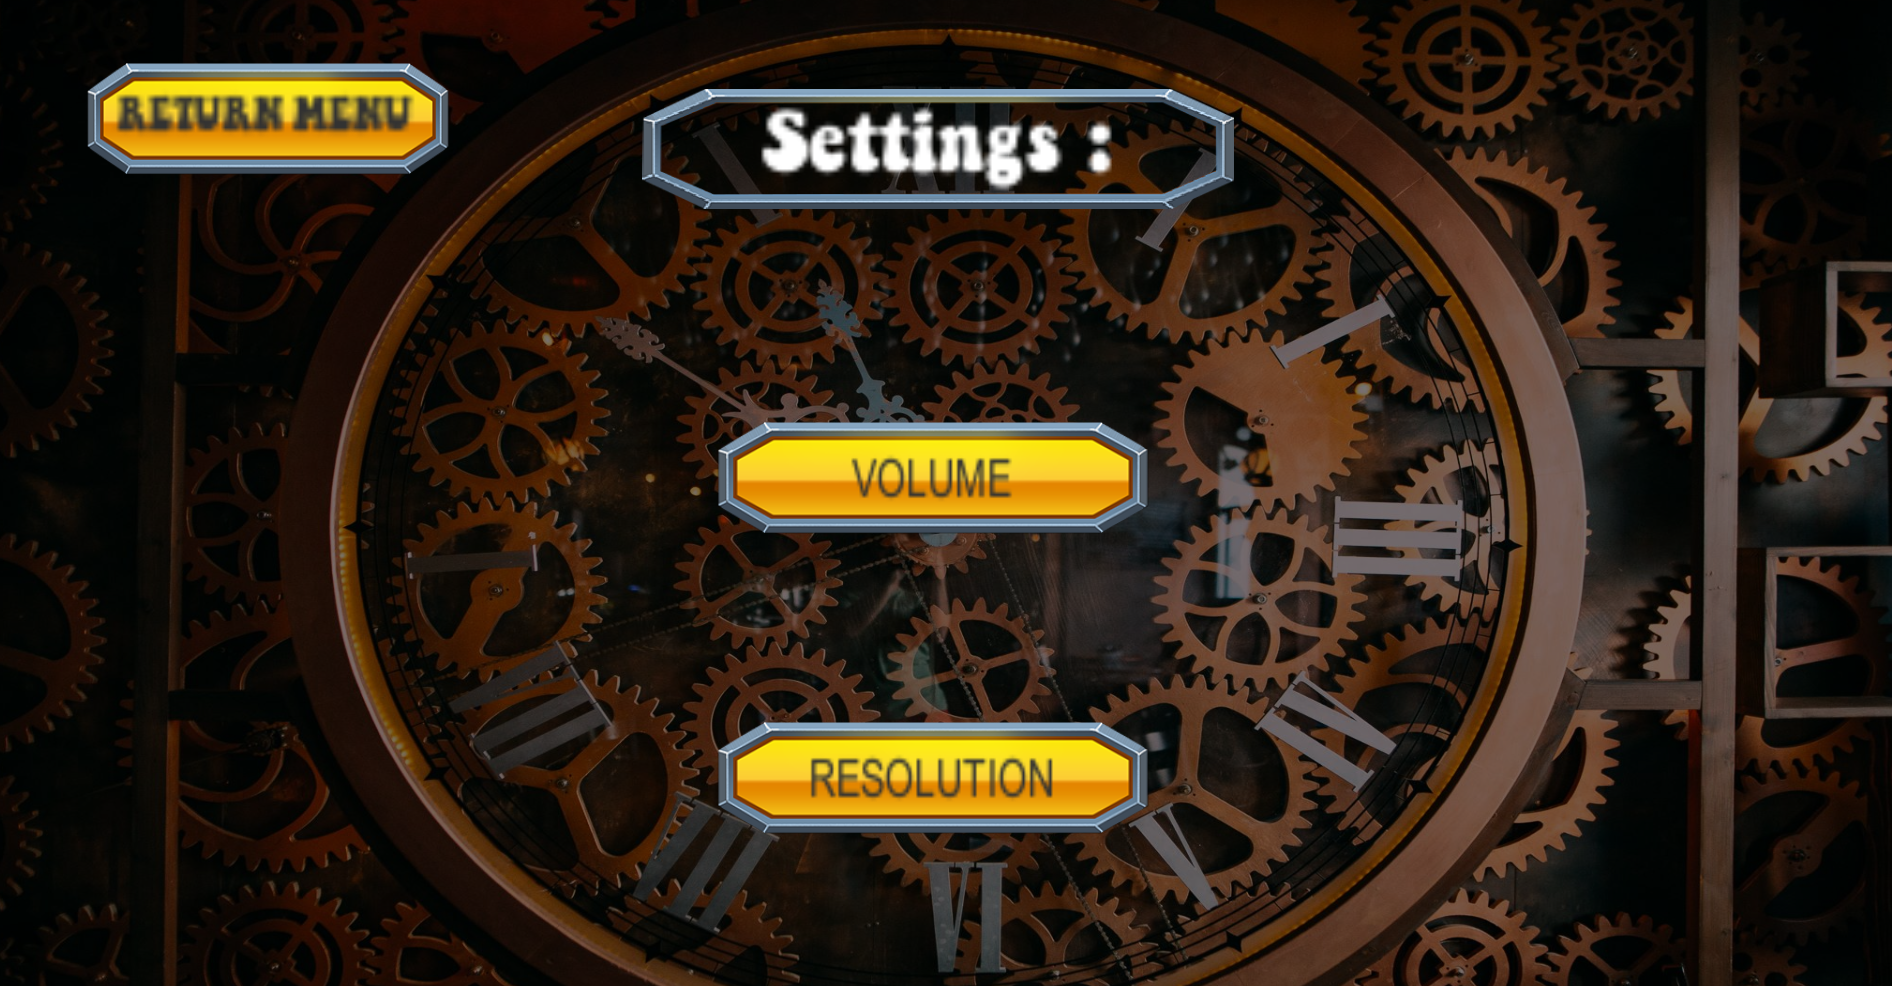
\includegraphics[scale=0.3]{images/settings.png}
		\caption{Menu Settings}
	\end{figure}
	
	\noindent Dans ce menu, vous avez 2 options :
	\begin{itemize}
		\item Volume : Régler le niveau sonore du jeu
		\item Resolution : Régler les paramètres d'écran
	\end{itemize}
	

	\subsection{Menu Volume}
	\begin{figure}[!ht]
		\centering
		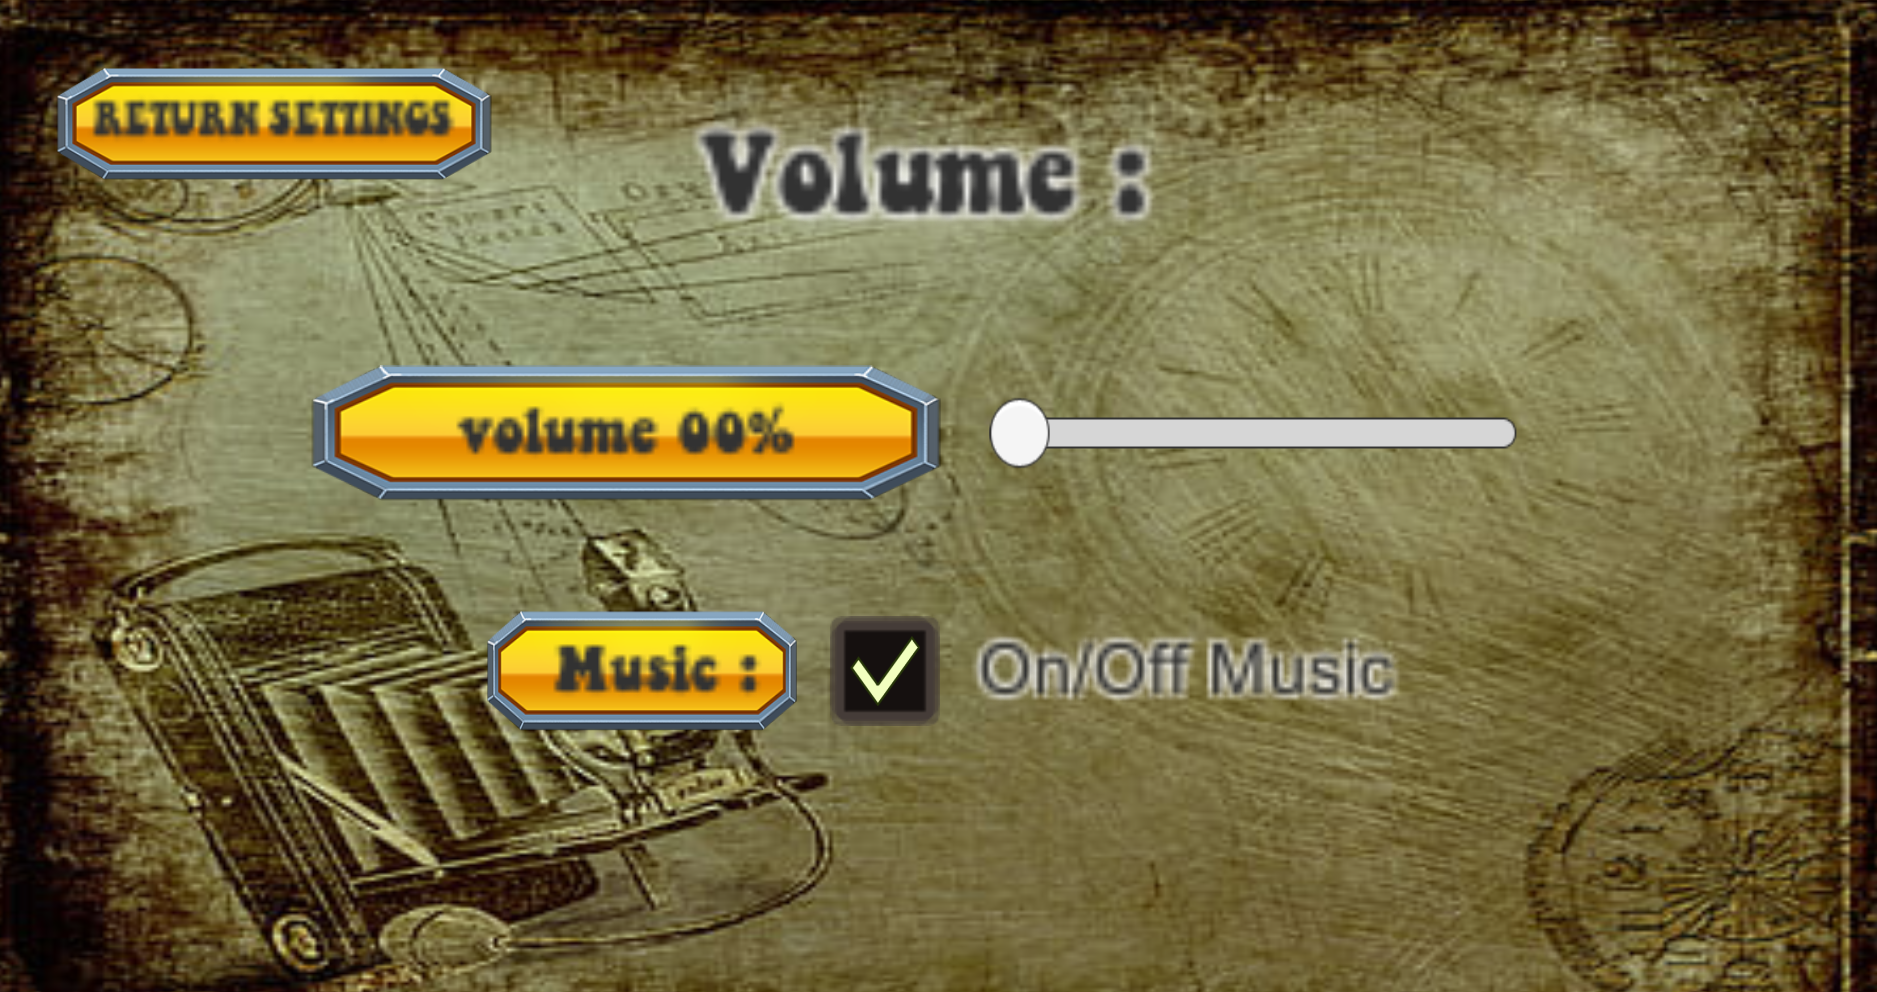
\includegraphics[scale=0.3]{images/volume.png}
		\caption{Menu Volume}
	\end{figure}
	
	\noindent Dans ce menu, vous avez 2 options : 
	\begin{itemize}
		\item La jauge de volume
		\item Activer ou désactiver la musique
	\end{itemize}
	
	\clearpage
	
	\subsection{Menu Résolution}
	\begin{figure}[!ht]
		\centering
		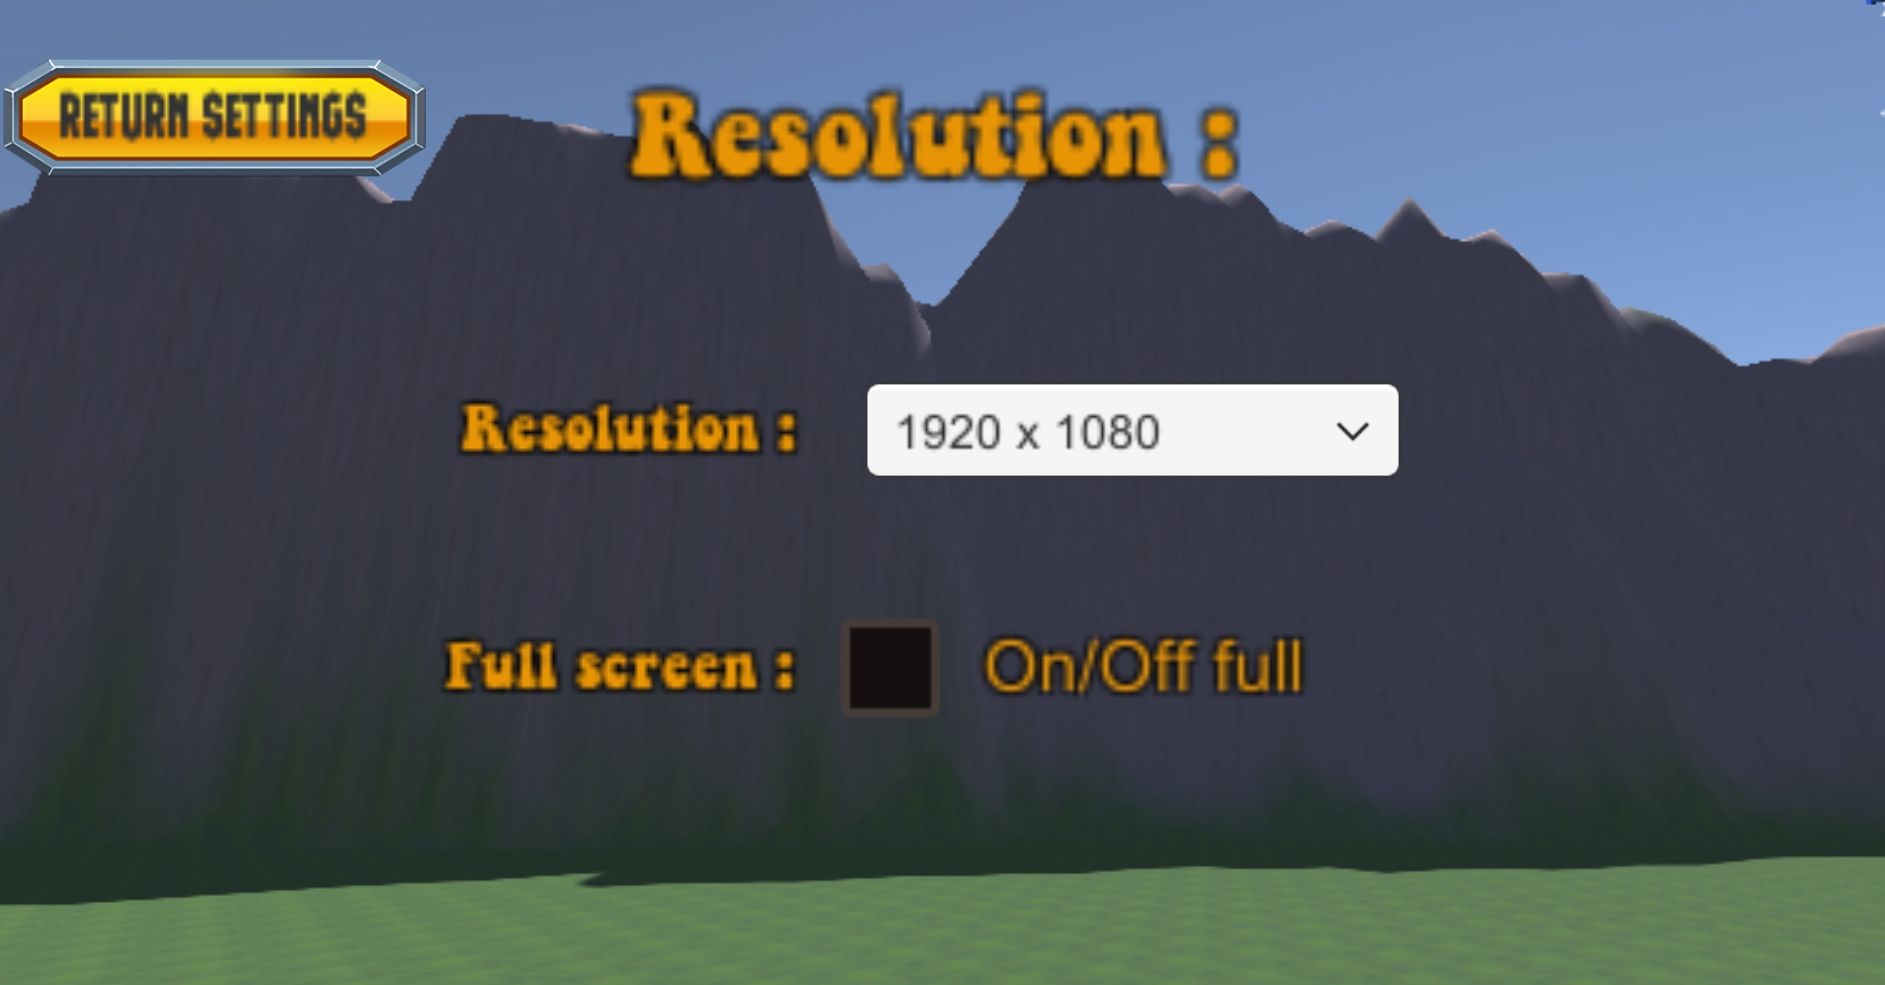
\includegraphics[scale=0.3]{images/resolution.png}
		\caption{Menu Résolution}
	\end{figure}
	
	\noindent Dans ce menu, vous avez 2 options :
	\begin{itemize}
		\item Resolution : Définir la résolution d'écran
		\item Full screen : Choisir de jouer en plein écran ou non
	\end{itemize}

	
	\subsection{Menu Play}
	\begin{figure}[!ht]
		\centering
		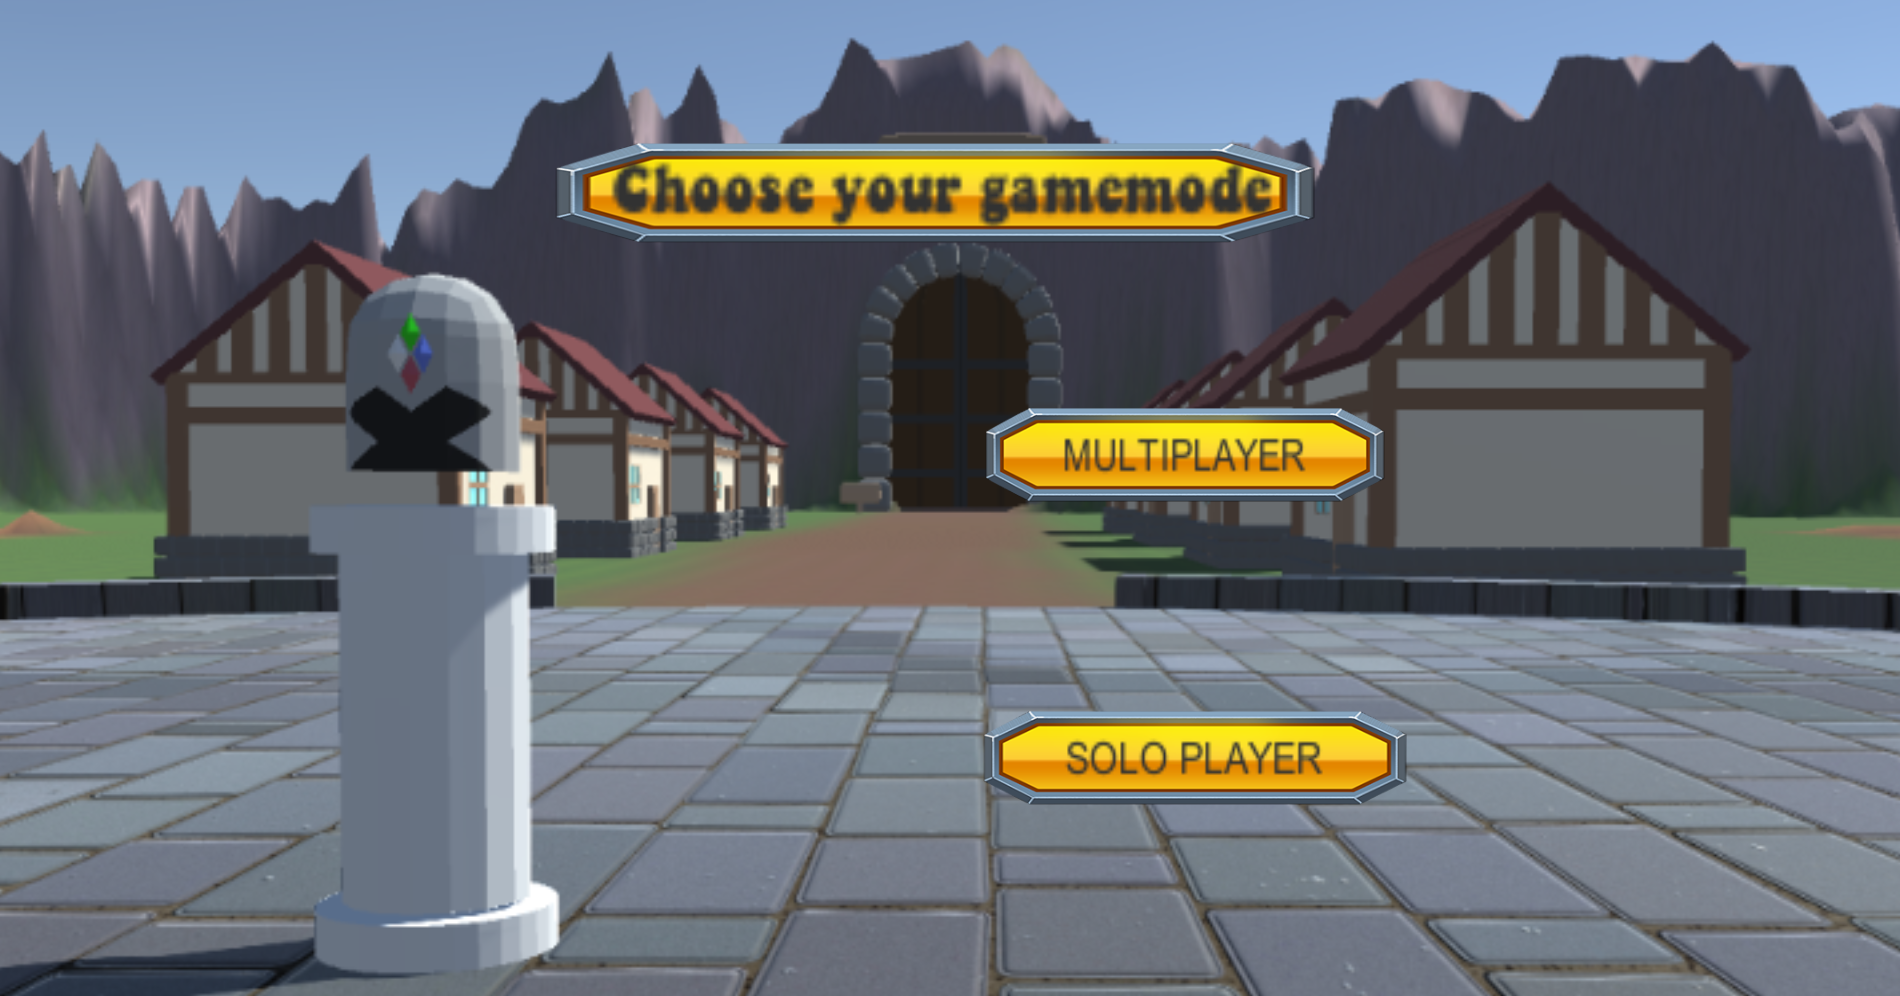
\includegraphics[scale=0.3]{images/play.png}
		\caption{Menu Play Game}
	\end{figure}
	
	\noindent Dans ce menu, vous avez 2 options :	
	
	\begin{itemize}
		\item Multiplayer : Jouer en multijoueur
		\item Solo Player : Jouer tout seul sans connexion
	\end{itemize}
	
	
	\subsection{Menu Multijoueur}
	\begin{figure}[!ht]
		\centering
		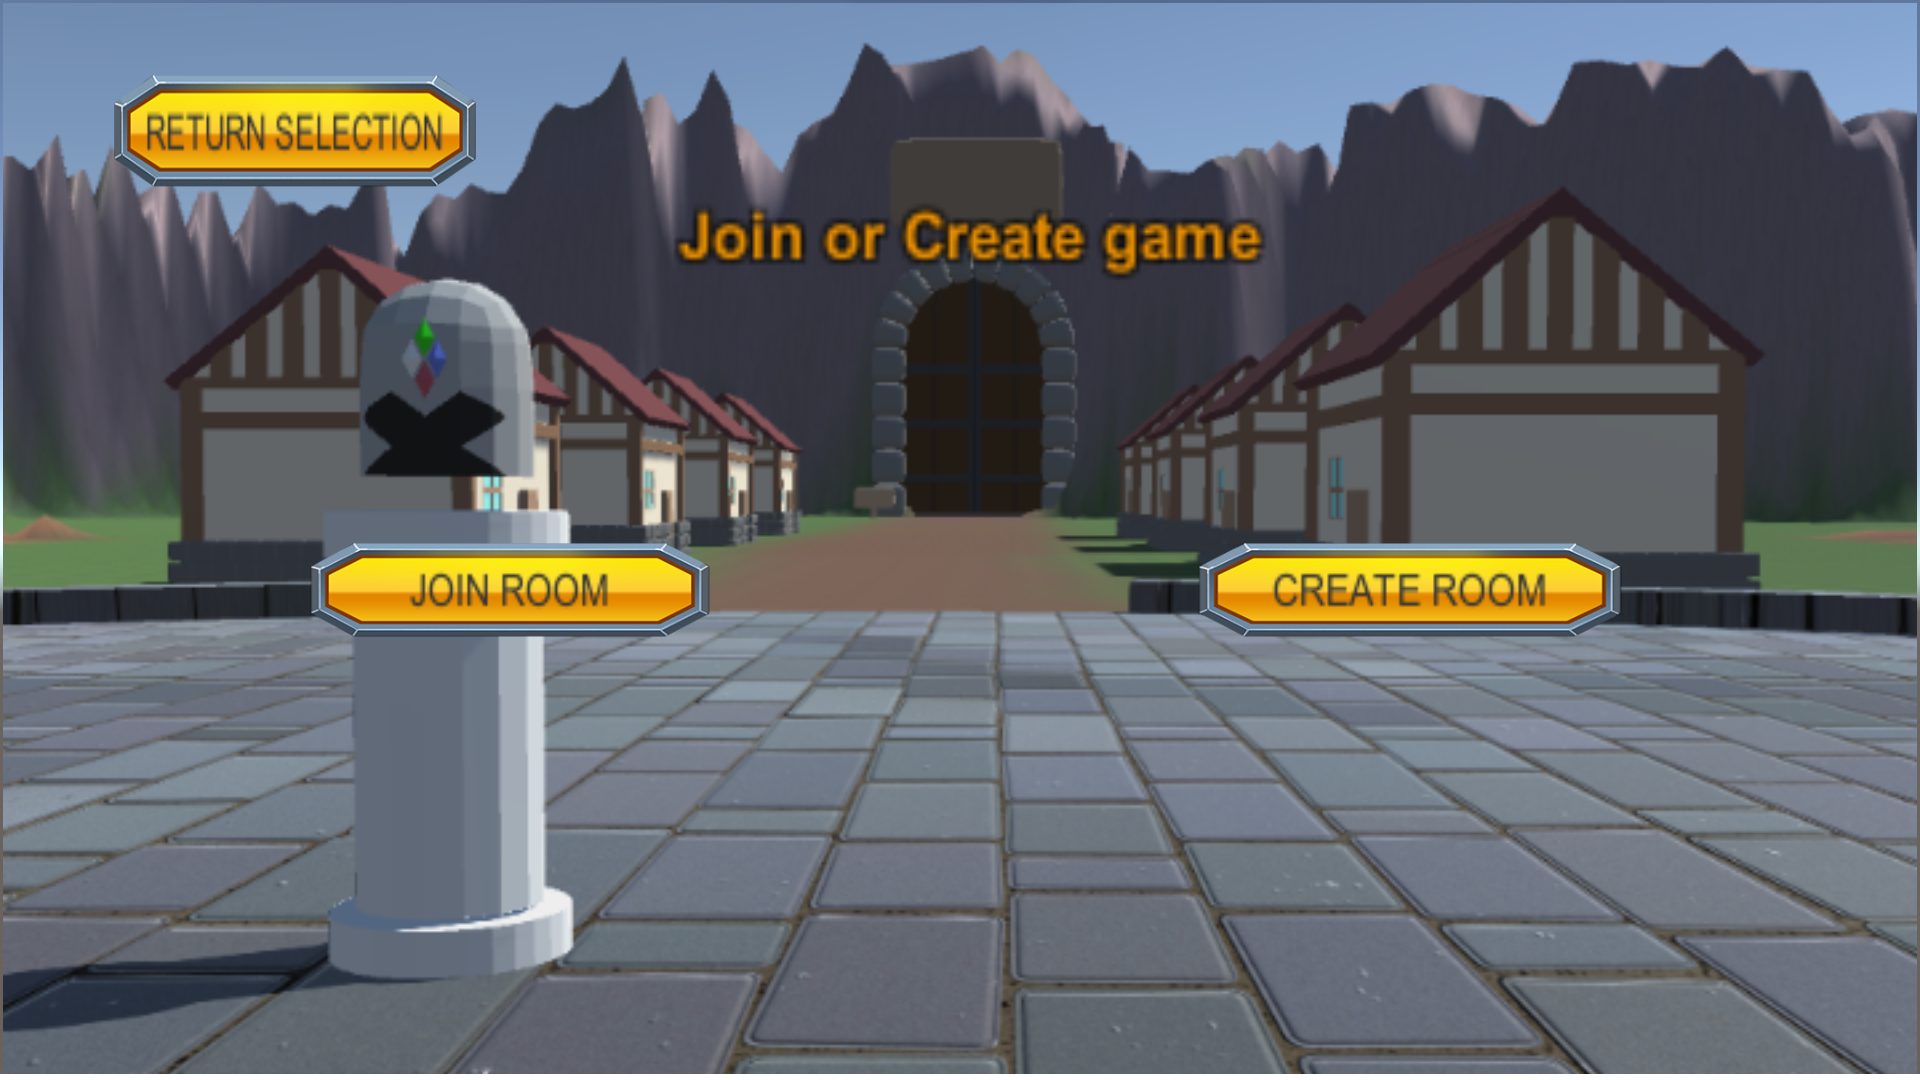
\includegraphics[scale=0.3]{images/multiplayer.png}
		\caption{Menu Multiplayer}
	\end{figure}
	
	\noindent Dans ce menu, vous avez 2 options :
	\begin{itemize}
		\item Join Room : Rejoindre une partie déjà existante
		\item Create Room : Créer une nouvelle partie
	\end{itemize}
	
	\clearpage	
	
	\subsection{Menu Create}
	\begin{figure}[!ht]
		\centering
		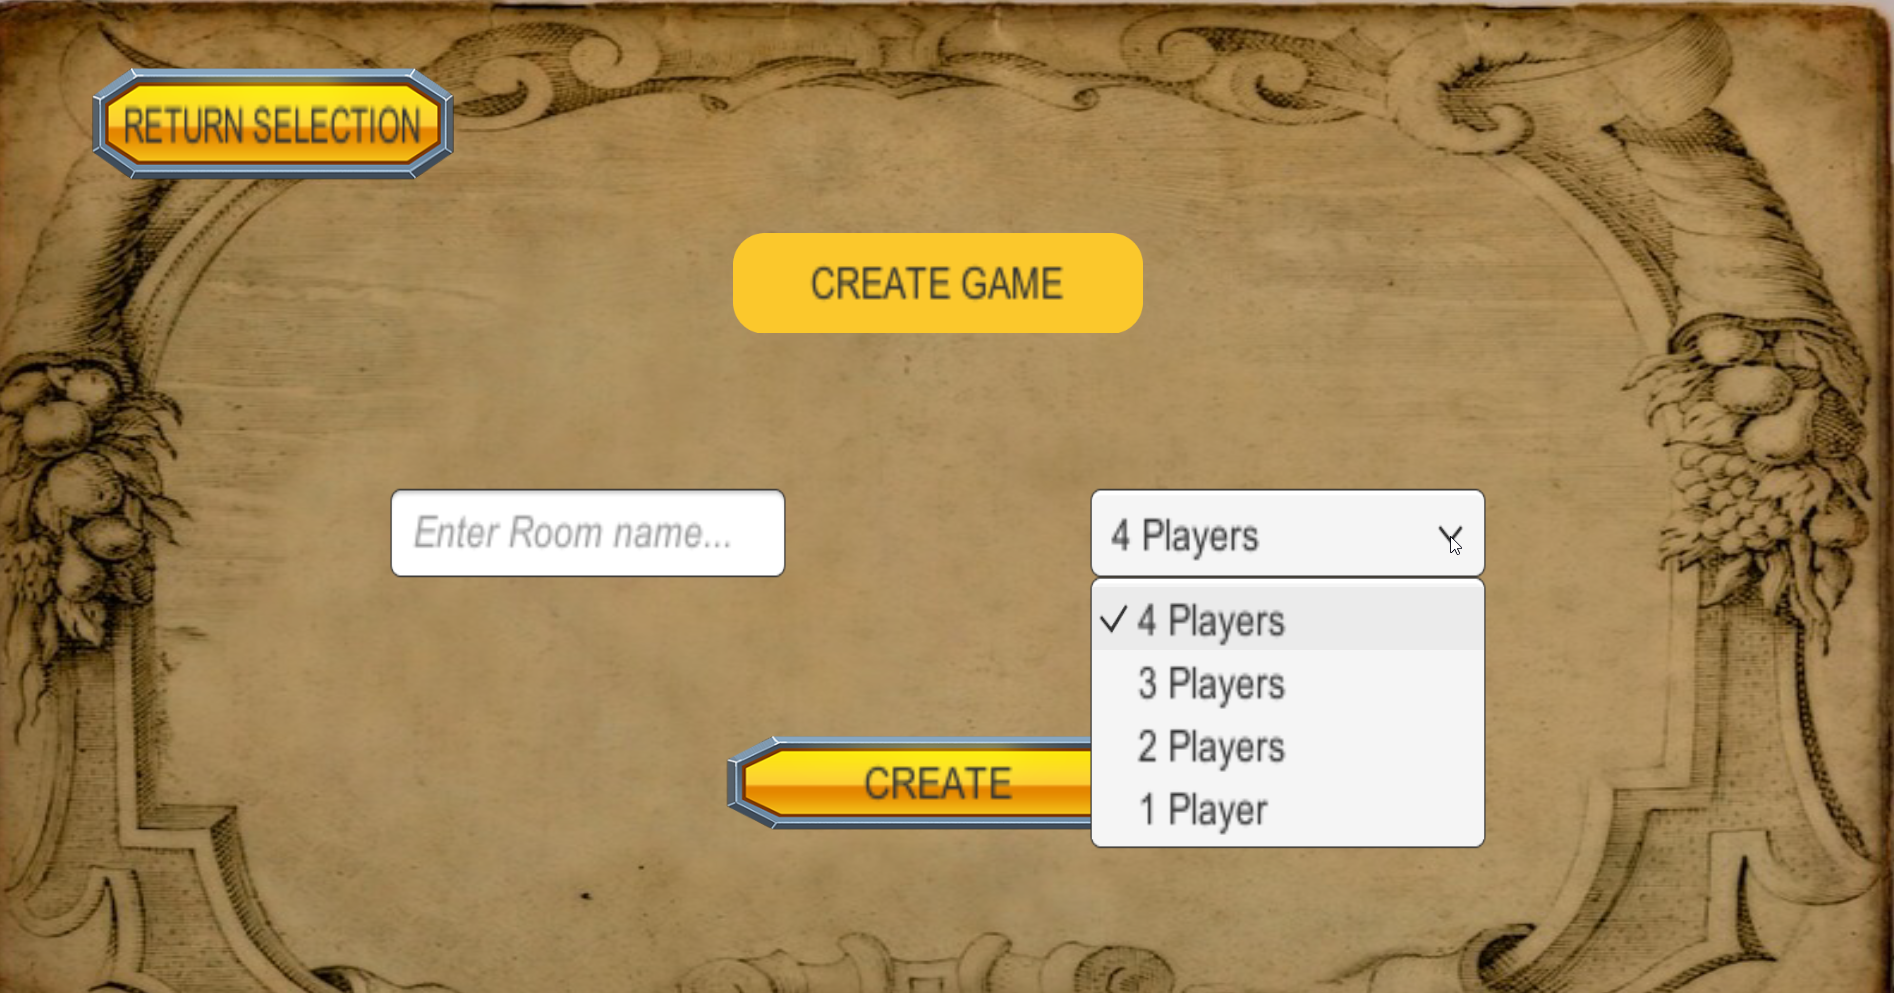
\includegraphics[scale=0.3]{images/create.png}
		\caption{Menu Create Game}
	\end{figure}
	
	\noindent Dans ce menu, vous avez 2 options :
	\begin{itemize}
		\item Le nom de la partie 
		\item Le nombre de joueurs maximum
	\end{itemize}
	
	\subsection{Menu Join}
	\begin{figure}[!ht]
		\centering
		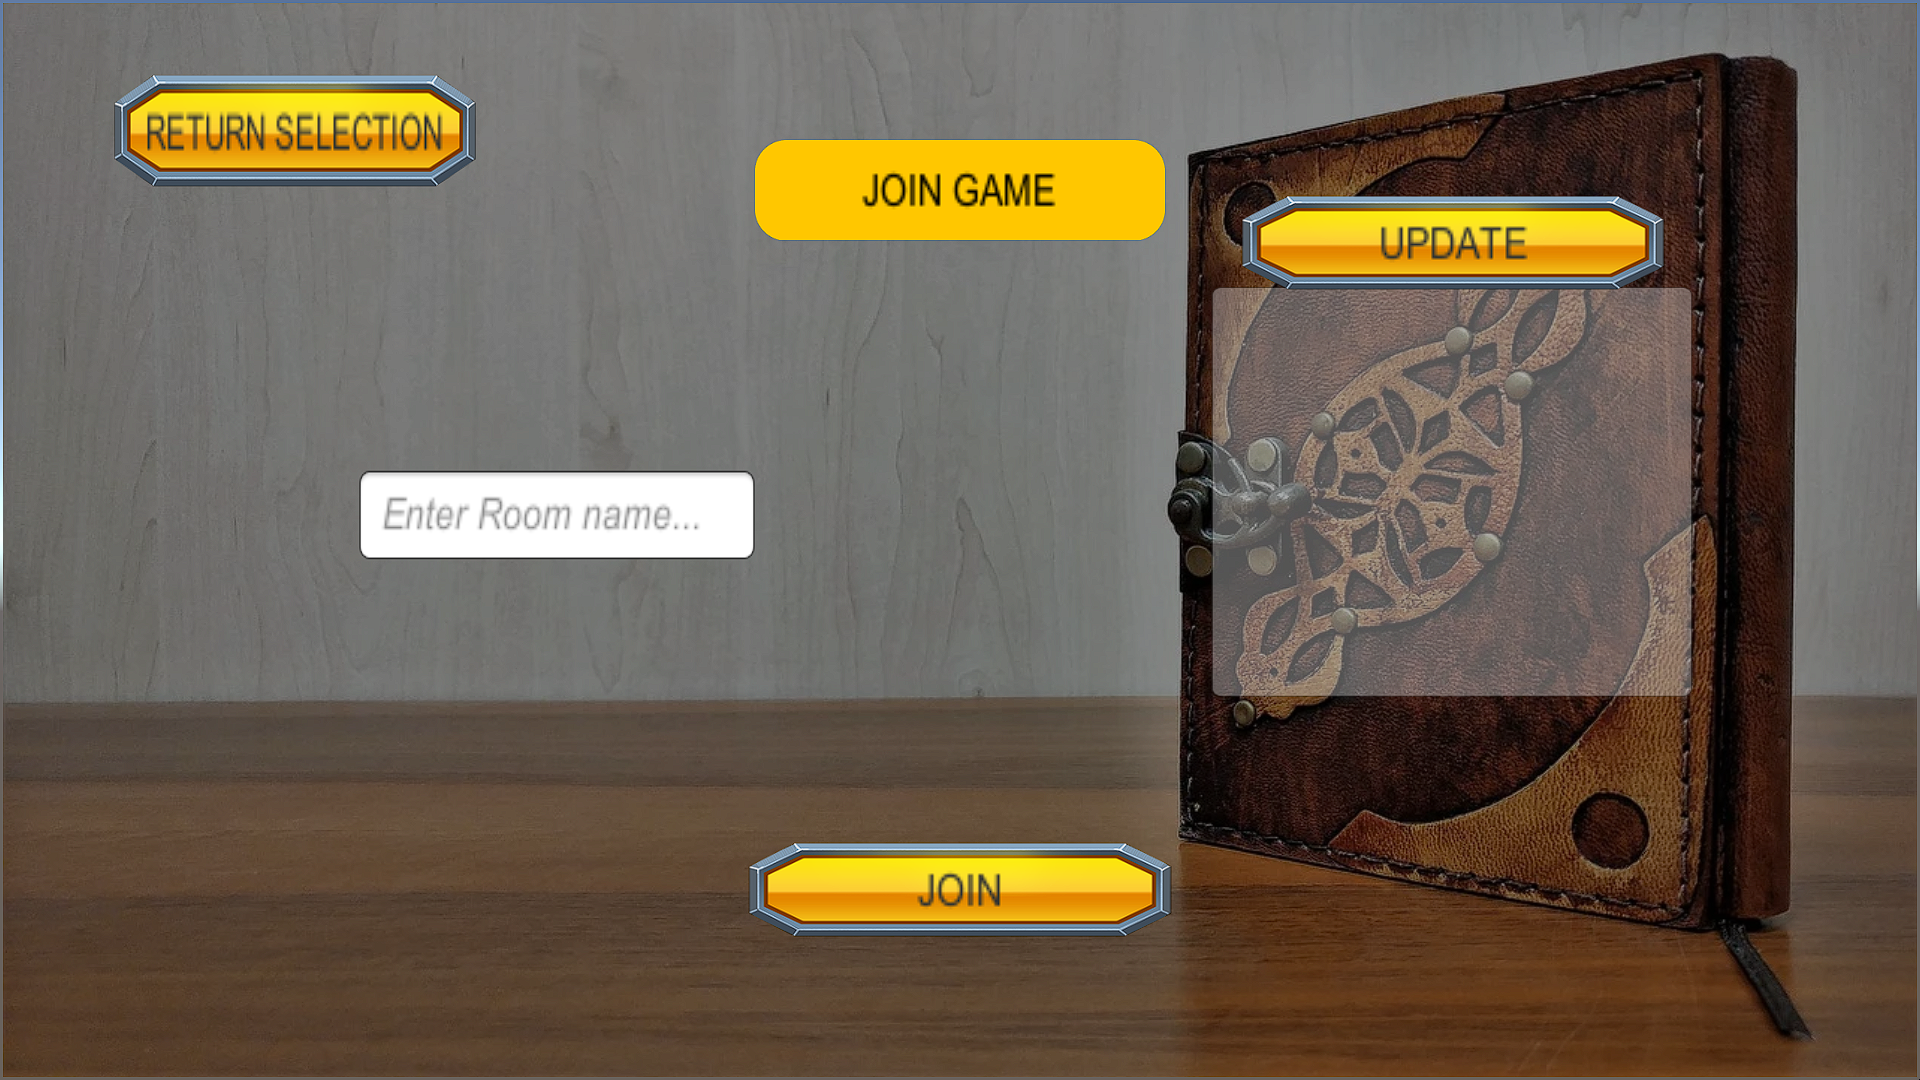
\includegraphics[scale=0.3]{images/join.png}
		\caption{Menu Join Game}
	\end{figure}
	
	\noindent Dans ce menu, vous pouvez :
	\begin{itemize}
		\item Entrer le nom de la partie à rejoindre
		\item Voir les noms des parties déjà existantes (avec Update pour rafraîchir)
	\end{itemize}
	
	\clearpage
	
	\subsection{Interface du jeu}
	\begin{figure}[!ht]
		\centering
		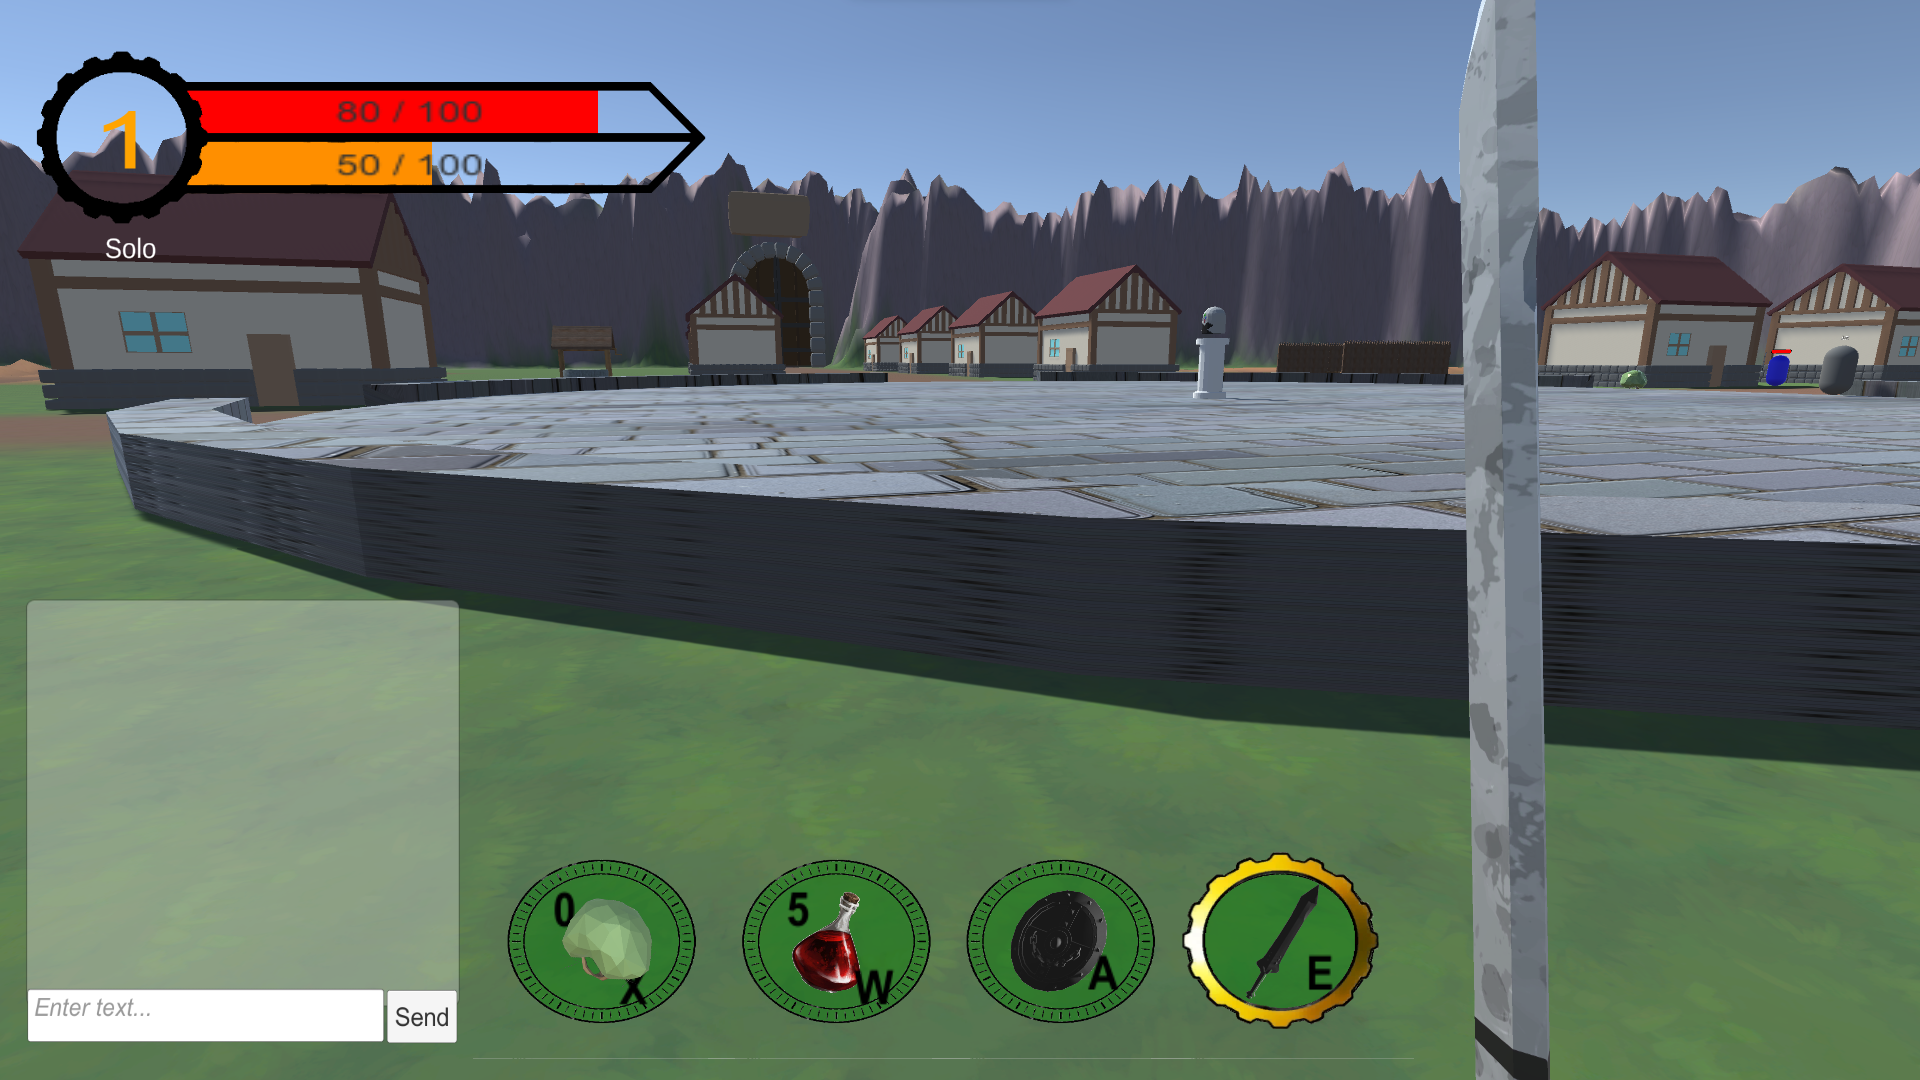
\includegraphics[scale=0.3]{images/hud.png}
		\caption{Interface du jeu}
	\end{figure}
	\begin{itemize}
		\item En haut à gauche :
		\begin{itemize}
			\item \textbf{Barre rouge} : Barre de vie
			\item \textbf{Barre orange} : Barre d'expérience
			\item \textbf{Numéro} : Niveau
		\end{itemize}
		\item En bas à gauche : Messagerie
		\item En bas : Objets
	\end{itemize}
	
	\subsection{Menu Pause}
	\begin{figure}[!ht]
		\centering
		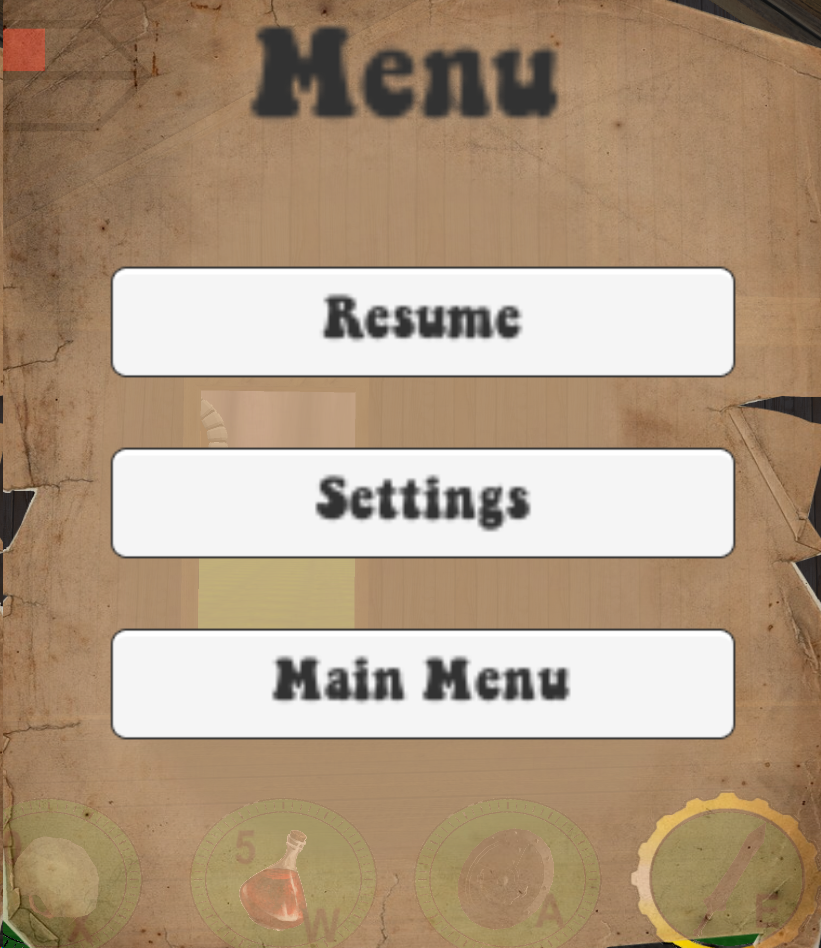
\includegraphics[scale=0.25]{images/pause.png}
		\caption{Menu Pause}
	\end{figure}
	
	\clearpage
	\section{Configuration des touches}
	\subsection{Déplacements}
	\begin{itemize}
		\item \boxed{\text{\textbf{Z}}} : Avancer
		\item \boxed{\text{\textbf{S}}} : Reculer
		\item \boxed{\text{\textbf{Q}}} : Gauche
		\item \boxed{\text{\textbf{D}}} : Droite
		\item \boxed{\text{\textbf{Maj}}} : Courir
		\item \boxed{\text{\textbf{Espace}}} : Sauter
		\item \boxed{\text{\textbf{Ctrl}}} : S'accroupir
	\end{itemize}
	
	\subsection{Inventaire}
	Vous pouvez accéder aux différentes catégories d'objets avec les touches suivantes : 
	\begin{itemize}
		\item \boxed{\text{\textbf{X}}} : Objets des quêtes
		\item \boxed{\text{\textbf{W}}} : Potions
		\item \boxed{\text{\textbf{A}}} : Bouclier
		\item \boxed{\text{\textbf{E}}} : Armes
		\item \boxed{\text{\textbf{Molette}}} : Naviguer dans une catégorie
	\end{itemize}
	
	\subsection{Interactions}
	\begin{itemize}
		\item \boxed{\text{\textbf{Entrée}}} : Activer/Désactiver le curseur pour cliquer sur la boîte de messagerie
		\item \boxed{\text{\textbf{F}}} : Interagir
		\item \boxed{\text{\textbf{Echap}}} : Afficher/Cacher le Menu Pause
		\item \boxed{\text{\textbf{Clic gauche}}} :
		\begin{itemize}
			\item Bouclier : Brandir
			\item Epée et Hache : Attaquer
		\end{itemize}
		\item \boxed{\text{\textbf{Clic droit}}} :
		\begin{itemize}
			\item Potions : Utiliser
			\item Arc et Bâton Magique : Attaquer
		\end{itemize}
	\end{itemize}
	
	\clearpage
	\section{Mécaniques de jeu avancées}
	\subsection{Wall-Run}
	Vous pouvez vous déplacer sur les murs.
	\\
	Pour ce faire vous pouvez sauter de profil vers un mur, puis vous déplacer avec les touches \boxed{\text{\textbf{Z}}} et \boxed{\text{\textbf{S}}} pour avancer ou reculer sur le mur.
	\\
	Note : Si vous avez sauté vers le mur en avançant, il faut utiliser la touche \boxed{\text{\textbf{Z}}} et pas \boxed{\text{\textbf{S}}}. Réciproquement si vous avez sauté en reculant.
	\subsection{Wall-Jump}
	\noindent Si vous êtes en train de glisser sur un mur, vous pouvez appuyer sur \boxed{\text{\textbf{Espace}}} pour sauter depuis le mur.
	
	\section{Changer de zone}
	Pour changer de zone, il vous suffit d'avancer vers la porte de la zone de votre choix. Chaque porte est différentiable par la couleur de sa pancarte.
	\\ 
	Exemple : Pancarte verte = Langdale.
	\begin{figure}[!h]
		\centering
		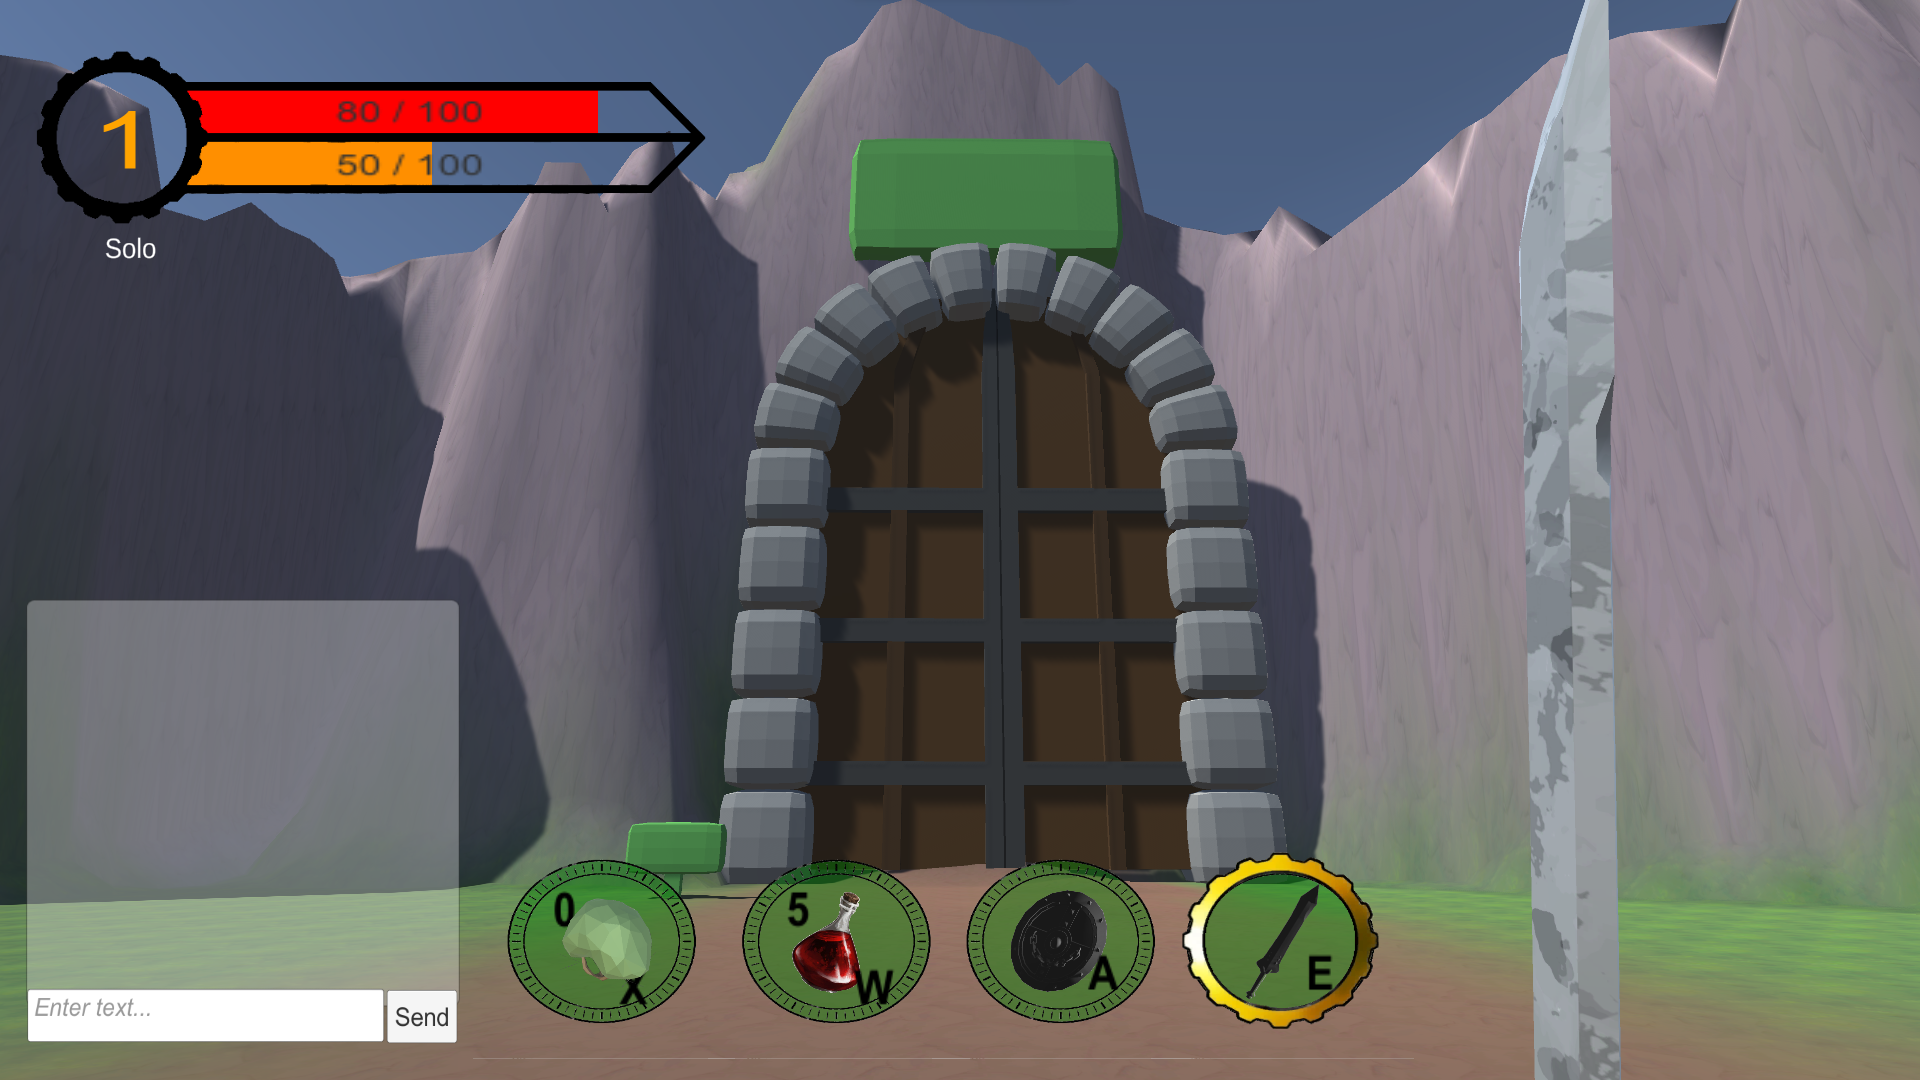
\includegraphics[scale=0.3]{images/porte_langdale.png}
		\caption{Porte de téléportation vers Langdale}
	\end{figure}
\end{document}